\subsection{第一问}
首先写一个生成高斯勒让德求积的系数和根的函数,即 Gauss.m, 通过输入整数 N 生成对应的系数和根。
再生成 $P_i$, 最后求出所有的 P 的和。整个代码在 exp1\_1.m 中。

通过计算得到对于所有的 n, \(\sum_{i=1}^{n+1}P_i=1\).
下面给出证明:
\begin{equation}
	\sum_{i=1}^{\mathrm{n}+1} P_{i}=\sum_{i=1}^{\mathrm{n}+1} \frac{W_{i} \sum_{j=0}^{n} \phi_{j}^{2}\left(x_{i}\right)}{n+1}
	= \frac{\sum_{i=1}^{\mathrm{n}+1}W_{i} \sum_{j=0}^{n} \phi_{j}^{2}\left(x_{i}\right)}{n+1}
\end{equation}
把分母单独提出来,即证分母等于 n+1 即可。
交换两求和符号顺序得
\begin{equation}
	\sum_{i=1}^{n+1}W_{i} \sum_{j=0}^{n} \phi_{j}^{2}\left(x_{i}\right)=\sum_{j=0}^{n}\sum_{i=1}^{n+1}W_i\phi_{j}^2(x_i)
\end{equation}
注意到里面的求和即是对每个$\phi_j$作 [0,1] 上的高斯求积,即值为 1.
而外面的求和做了 n+1 次,因此分母的和为 n+1.
所以最终求得\(\sum_{i=1}^{n+1}P_i=1\). \hfill \(\qedsymbol\)

\subsection{第二问}
观察需要优化的式子即可知道这是一个二次型最优化,而二次型优化的标准式为
\begin{equation}
	\min _{x} \frac{1}{2} x^{T} H x+f^{T} x
\end{equation}
则我们只需要算出二次型优化中的 $\mathbf{H,f}$即可.
\begin{equation}
	\sum_{i=1}^{n+1}\left|\sum_{j=0}^{n} c_{j} \phi_{j}\left(x_{i}\right)-f\left(x_{i}\right)\right|^{2}=
	|\mathbf{\Phi} \mathbf {\hat{c}}-\mathbf F|^2
\end{equation}
这里 $\mathbf{\Phi}$ 的每个元素为 $\Phi_{ij}=\phi _{j-1}(x_i)$, 且 \(\mathbf{\Phi}\) 为 \((n+1)\times(n+1)\) 的矩阵。
\(\mathbf{\hat{c},F}\) 分别代表系数与每个 \(x_i\) 对应的 \(f\) 的值。

把上面的式子变为二次型标准型:
\begin{equation}
	|\mathbf{\Phi} \mathbf{\hat{c}}-\mathbf F|^2=(\mathbf{\Phi} \mathbf {\hat{c}}-\mathbf F)'(\mathbf{\Phi} \mathbf {\hat{c}}-\mathbf F)=
	(\mathbf{\hat{c}}'\mathbf{\Phi}'-\mathbf{F}')(\mathbf{\Phi} \mathbf {\hat{c}}-\mathbf F)=
	\mathbf{\hat{c}}'\mathbf{\Phi}'\mathbf{\Phi}\mathbf{\hat{c}}-2\mathbf{F}'\mathbf{\Phi}\mathbf{\hat{c}}+\mathbf{F}'\mathbf{F}
\end{equation}
则令 \(\mathbf{H}=\mathbf{\Phi'\Phi},\ \mathbf{f}=-\mathbf{\Phi' F}\).
在代码中用循环生成 \(\mathbf{\Phi}\), 把它存在 legendre\_matrix 中。
之后相继生成 \(\mathbf{H},\ \mathbf{f}\), 并存在 H 和 f\_value 中。
用 'quadprog' 函数对其进行优化,即可得到 \(\mathbf{\hat{c}}\).

将 \(c_k\) 与 \(\sum_{i=1}^{n+1}f\left(x_{i}\right) w_{i} \phi_{k}\left(x_{i}\right)\) 进行比较,发现
\begin{equation}
	c_k=\sum_{i=1}^{n+1}f\left(x_{i}\right) w_{i} \phi_{k}\left(x_{i}\right),\ k=0,1\dots n
\end{equation}

相关程序在 exp1\_23.m 中。
下面给出数学证明。

首先注意到 \(\mathbf{H}\) 必定为正定矩阵,因为 \(\mathbf{\Phi'\Phi}\) 的所有特征值必定都大于 0.
则该二次型的最优解为 \(\mathbf{\hat{c}}=\mathbf{H}^{-1}\mathbf{(-F)}\), 即 \(\mathbf{\hat{c}}=\mathbf{\Phi'\Phi}^{-1}\mathbf{\Phi' F}\).
接下来只需证明 \(\mathbf{\Phi'\Phi}^{-1}\mathbf{\Phi' F}=\mathbf{\Phi'}\text{diag}(\mathbf{W})F\) 即可。
其中 \(\text{diag}(\mathbf{W})\) 指的是对角线全为 \(\mathbf{W}\) 的元素的 \((n+1)\times (n+1)\) 的矩阵。

可以验证 \(\mathbf{\Phi'}\text{diag}(\mathbf{W})\mathbf{F}\) 的第 k 个元素为 \(\sum_{i=1}^{n+1}f\left(x_{i}\right) w_{i} \phi_{k}\left(x_{i}\right)\).

下面接着证明 \(\mathbf{\Phi'\Phi}^{-1}\mathbf{\Phi' F}=\mathbf{\Phi'}\text{diag}(\mathbf{W})\mathbf{F}\).

\begin{equation}
	\begin{aligned}
		\mathbf{\Phi'\Phi}^{-1}\mathbf{\Phi' F} &=\mathbf{\Phi'}\text{diag}(\mathbf{W})\mathbf{F} \\
		\mathbf{\Phi' F} &=\mathbf{\Phi'\Phi}\mathbf{\Phi'}\text{diag}(\mathbf{W})\mathbf{F} \\
		\mathbf{F} &=\mathbf{\Phi}\mathbf{\Phi'}\text{diag}(\mathbf{W})\mathbf{F} \\
		\mathbf{I} &=\mathbf{\Phi}\mathbf{\Phi'}\text{diag}(\mathbf{W})
	\end{aligned}
\end{equation}

\vspace{1em}
第三个等式能消去 \(\mathbf{\Phi'}\) 的原因是因为可逆,第四个等式能消去 \(\mathbf{F}\) 的原因是 \(\mathbf{\Phi},\text{diag}(\mathbf{W})\) 都与 \(\mathbf{F}\) 无关
且 \(\mathbf{F}\) 可以几乎取任意的值(由函数 \(f(x)\) 而定)。

最后 \(\mathbf{\Phi}\mathbf{\Phi'}\text{diag}(\mathbf{W})\) 即是 \(\int_{-1}^{1} \phi_{i}(x) \phi_{j}(x) d x\).
则对角元上 \(i=j\), 为 1,非对角元上 \(i\neq j\), 为 0.
因此,最后等于单位矩阵,因此,上式的第四个等式成立,从而第一个式子成立,即猜想正确。\hfill\(\qedsymbol\)

\subsection{第三问}
紧接着上述的程序(即相关代码在 exp1\_23.m 中)。
\(\Phi_{i}\) 即是 \(\mathbf{\Phi}\) 的第 i 行的数据,即 legendre\_matrix 的第 i 行。
之后开始每次迭代,把每次计算出的误差存入变量 e 中。
这里并没有计入第一次随机生成 c 时的误差,因此 e 为 \((n+1)\times 1\) 的向量。
下面分别是 \(f(x)=x,\ f(x)=\sin(x),\ f(x)=e^x\) 的误差图像。(此时 n 都取的是 10)
\begin{figure}[H]
	\centering
	\begin{subfigure}[t]{0.3\textwidth}
		\centering
		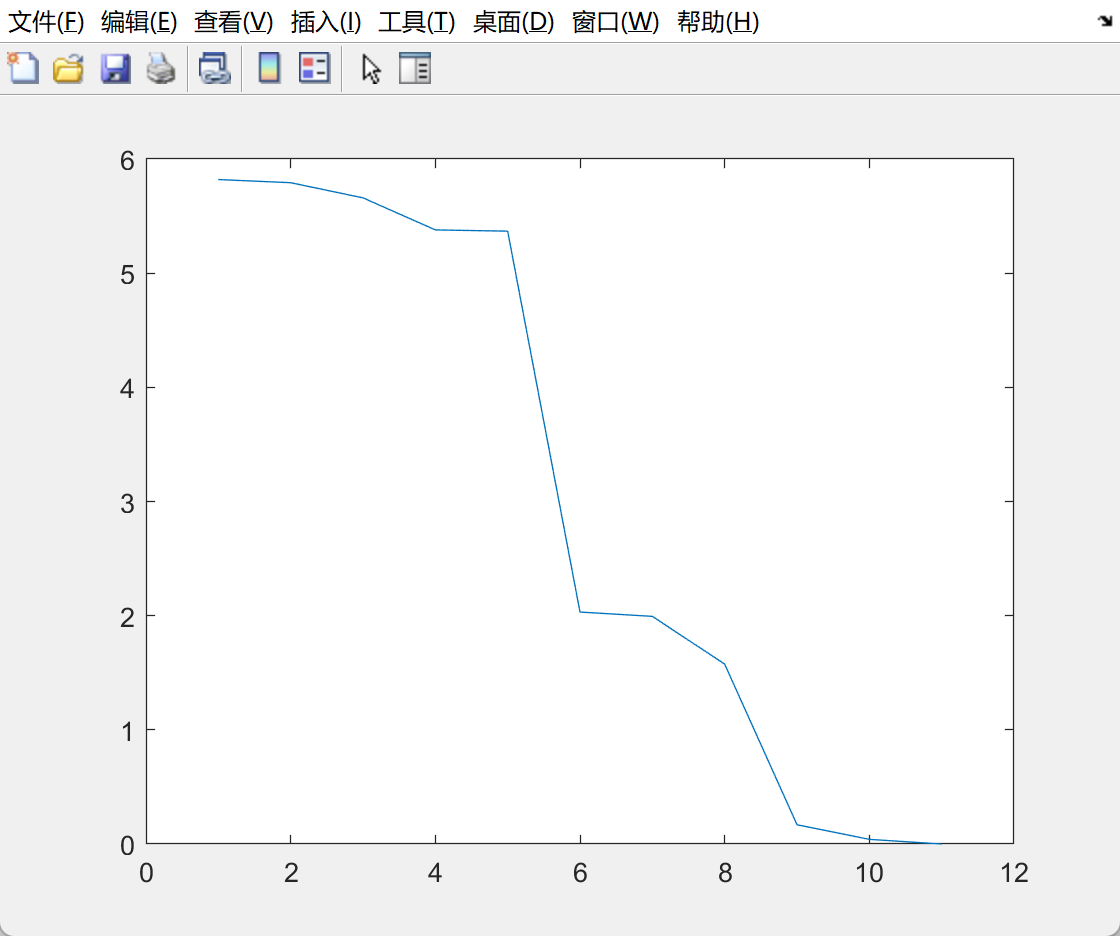
\includegraphics[width=\textwidth]{./picture/exp1_3_1}
		\caption{}
		\label{fig:a}
	\end{subfigure}
	\begin{subfigure}[t]{0.3\textwidth}
		\centering
		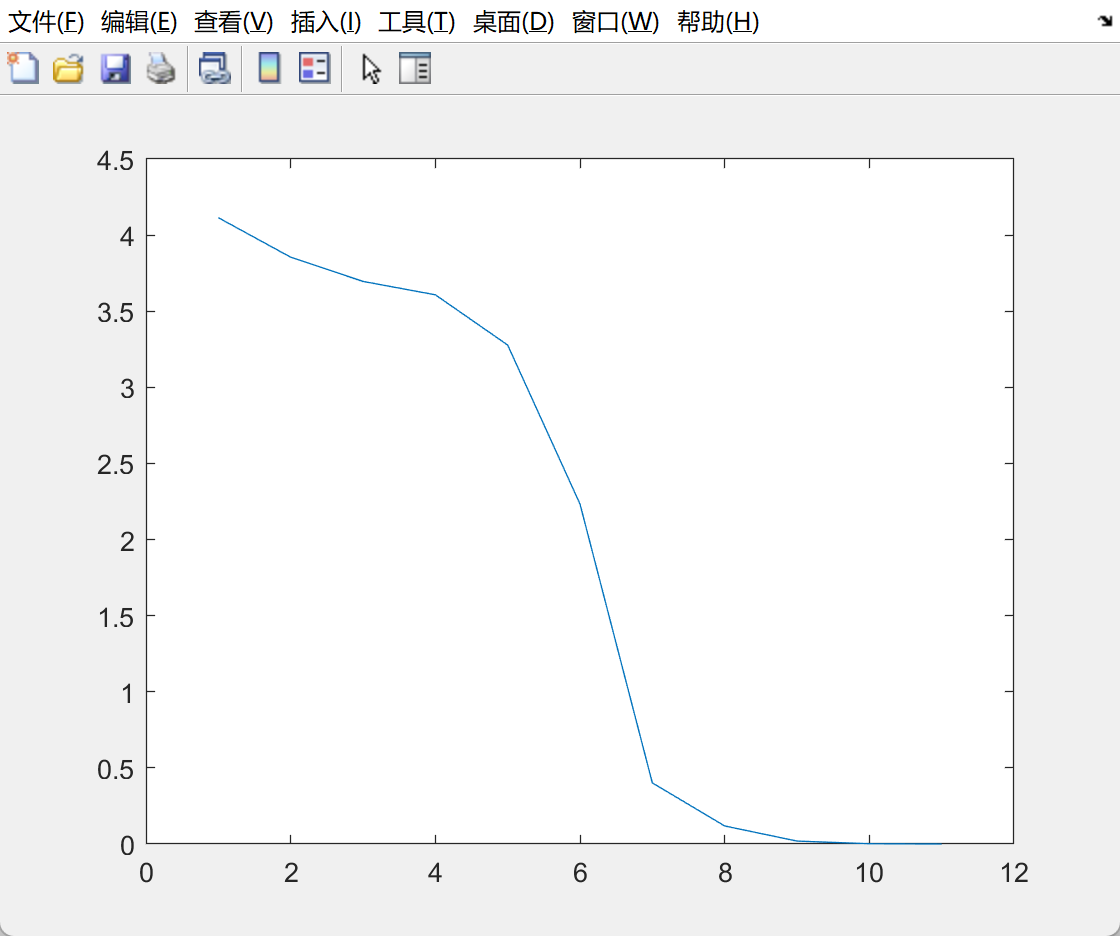
\includegraphics[width=\textwidth]{./picture/exp1_3_2}
		\caption{}
		\label{fig:b}
	\end{subfigure}
	\begin{subfigure}[t]{0.3\textwidth}
		\centering
		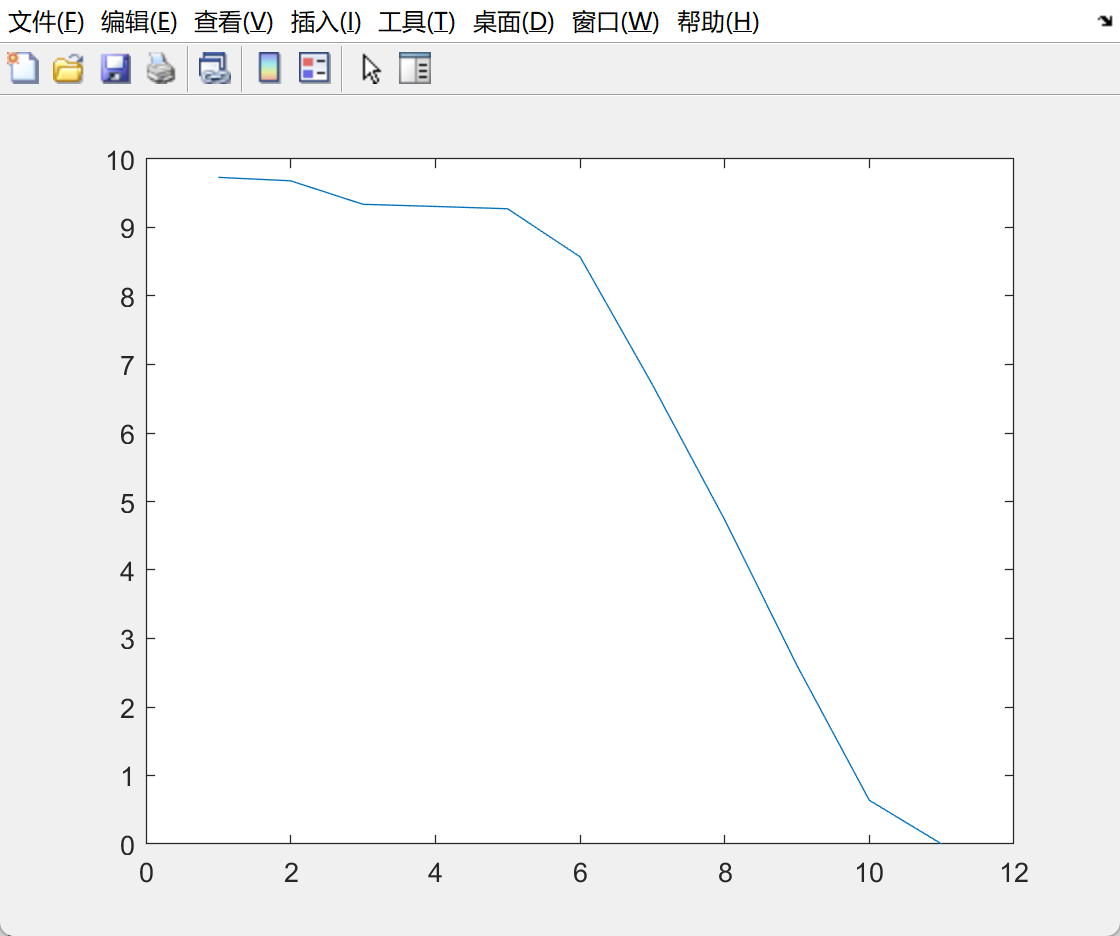
\includegraphics[width=\textwidth]{./picture/exp1_3_3}
	\end{subfigure}
\end{figure}

可以看出误差都呈下降趋势,且当 \(i=n+1\) 时,误差非常小,达到了 \(10^{-20}\) 的数量级或者更小。
因此,猜想是当 \(i=n+1\) 时,\(\boldsymbol{C}^{(i)}\) 几乎达到真实值 \(\mathbf{\hat{c}}\).

下面给出证明:

注意到递推式与牛顿法的形式很相近,因此考虑用牛顿法证明该数列收敛且收敛到 \(\mathbf{\hat{c}}\).
牛顿法的原始形式为
\begin{equation}
	x_{n+1}=x_{n}-\frac{f\left(x_{n}\right)}{f^{\prime}\left(x_{n}\right)}
\end{equation}

\hspace{2em}
令 \(g(\mathbf{\hat{c}})=(\mathbf{c}\cdot \Phi_i- f(x_i))\Phi_i\), 则
\(\frac{\partial g}{\partial \mathbf{\hat c}} =\Phi_i \cdot \Phi_i=||\Phi_i||^2\), 正好等于分母。

因此该递推式收敛的条件为分子有零点,即
\begin{equation}
	g(\mathbf{\hat{c}})=(\mathbf{c}\cdot \Phi_i- f(x_i))\Phi_i \label{eq:eq1}
\end{equation}
有零点。

注意到 \[\mathbf{\hat{c}}=\mathbf{\Phi'\Phi}^{-1}\mathbf{\Phi F'}\]
两边同时左乘 \(\mathbf{\Phi}\) 得
\[\mathbf{\Phi}\mathbf{\hat{c}}=\mathbf{\Phi}\mathbf{\Phi'\Phi}^{-1}\mathbf{\Phi F'}\]
因为 \(\Phi\) 是可逆的,因此括号中的项可以提出,得
\[\mathbf{\Phi}\mathbf{\hat{c}}=\mathbf{\Phi}\mathbf{\Phi}^{-1}\mathbf{\Phi'}^{-1}\mathbf{\Phi' F}\\
\mathbf{\Phi}\mathbf{\hat{c}}=\mathbf{F}\]
所以 \(\mathbf{F}\) 的第 i 个元素为 \(\mathbf{\Phi}\) 的第 i 行乘以 \(\mathbf{\hat{c}}\), 即 \(\Phi_i \cdot \mathbf{\hat{c}}\).

所以\eqref{eq:eq1}式有解,也就是说 \(\mathbf{c}^{(i)}\) 收敛于 \(\mathbf{\hat{c}}\).